%%--------------------------------------------------------------------------------------------------------------------%%
\subsection{A three-dimensional experiment: the Hessenthaler flap}\label{sec:hessenthaler_m}
%%--------------------------------------------------------------------------------------------------------------------%%
% DRAFT (13 Nov 2026), added for Philip to judge fit; may be dropped depending
% on the outcome of the QM and partitioned runs. Abstract, introduction and
% conclusions deliberately not updated. To remove: delete the \input line at
% the end of sectionAccuracyCost.tex.
% Data: paper-data/hessenthaler/ (tip histories, window summary, centrelines,
% voxel profiles); scripts figures/scripts/hessenthaler_results.py and the
% hessenthalerFsi validation driver; QM runs MeluXina philip-hvqm/runs/rF*_S2_
% qm_b02LUST_T45 (build-bf697 = 517a44921 + #697 fix); partitioned runs UCD
% Sonic /scratch/pcardiff/hv/P_rF*_LUST_b02 (206437983 + PR 676, 64896b0a5).
\todo{Draft for a decision on whether to keep this case. Incomplete: the QM runs on rF1 (at $t = 15.4\,\mathrm{s}$) and rF2 (at $t = 8.7\,\mathrm{s}$) and the partitioned run on rF2 (at $t = 42.4\,\mathrm{s}$) are still running, so only rF0 is compared over the closing window; protocol timings of both couplings on one machine are not yet taken; the abstract, introduction and conclusions do not mention this case yet.}

The cases above are two-dimensional and have numerical references.
The experiment of~\citet{Hessenthaler2017a} adds what they lack: a three-dimensional flow through a branching vessel geometry, a flap that deflects by a quarter of its length under combined buoyancy and flow, and measurements of the flap position and of the velocity field by magnetic resonance imaging (MRI) (Figure~\ref{fig:hessenthaler_3d}).
It has no numerical reference solution; it is used here to compare the two couplings on a large three-dimensional problem and, separately, to check that both agree with the measurements as well as the measurements allow.
Its verification by self-convergence of the partitioned solution is the subject of the companion paper~\citep{CardiffFSIVerification2026}.

\begin{figure}[htbp]
	\centering
	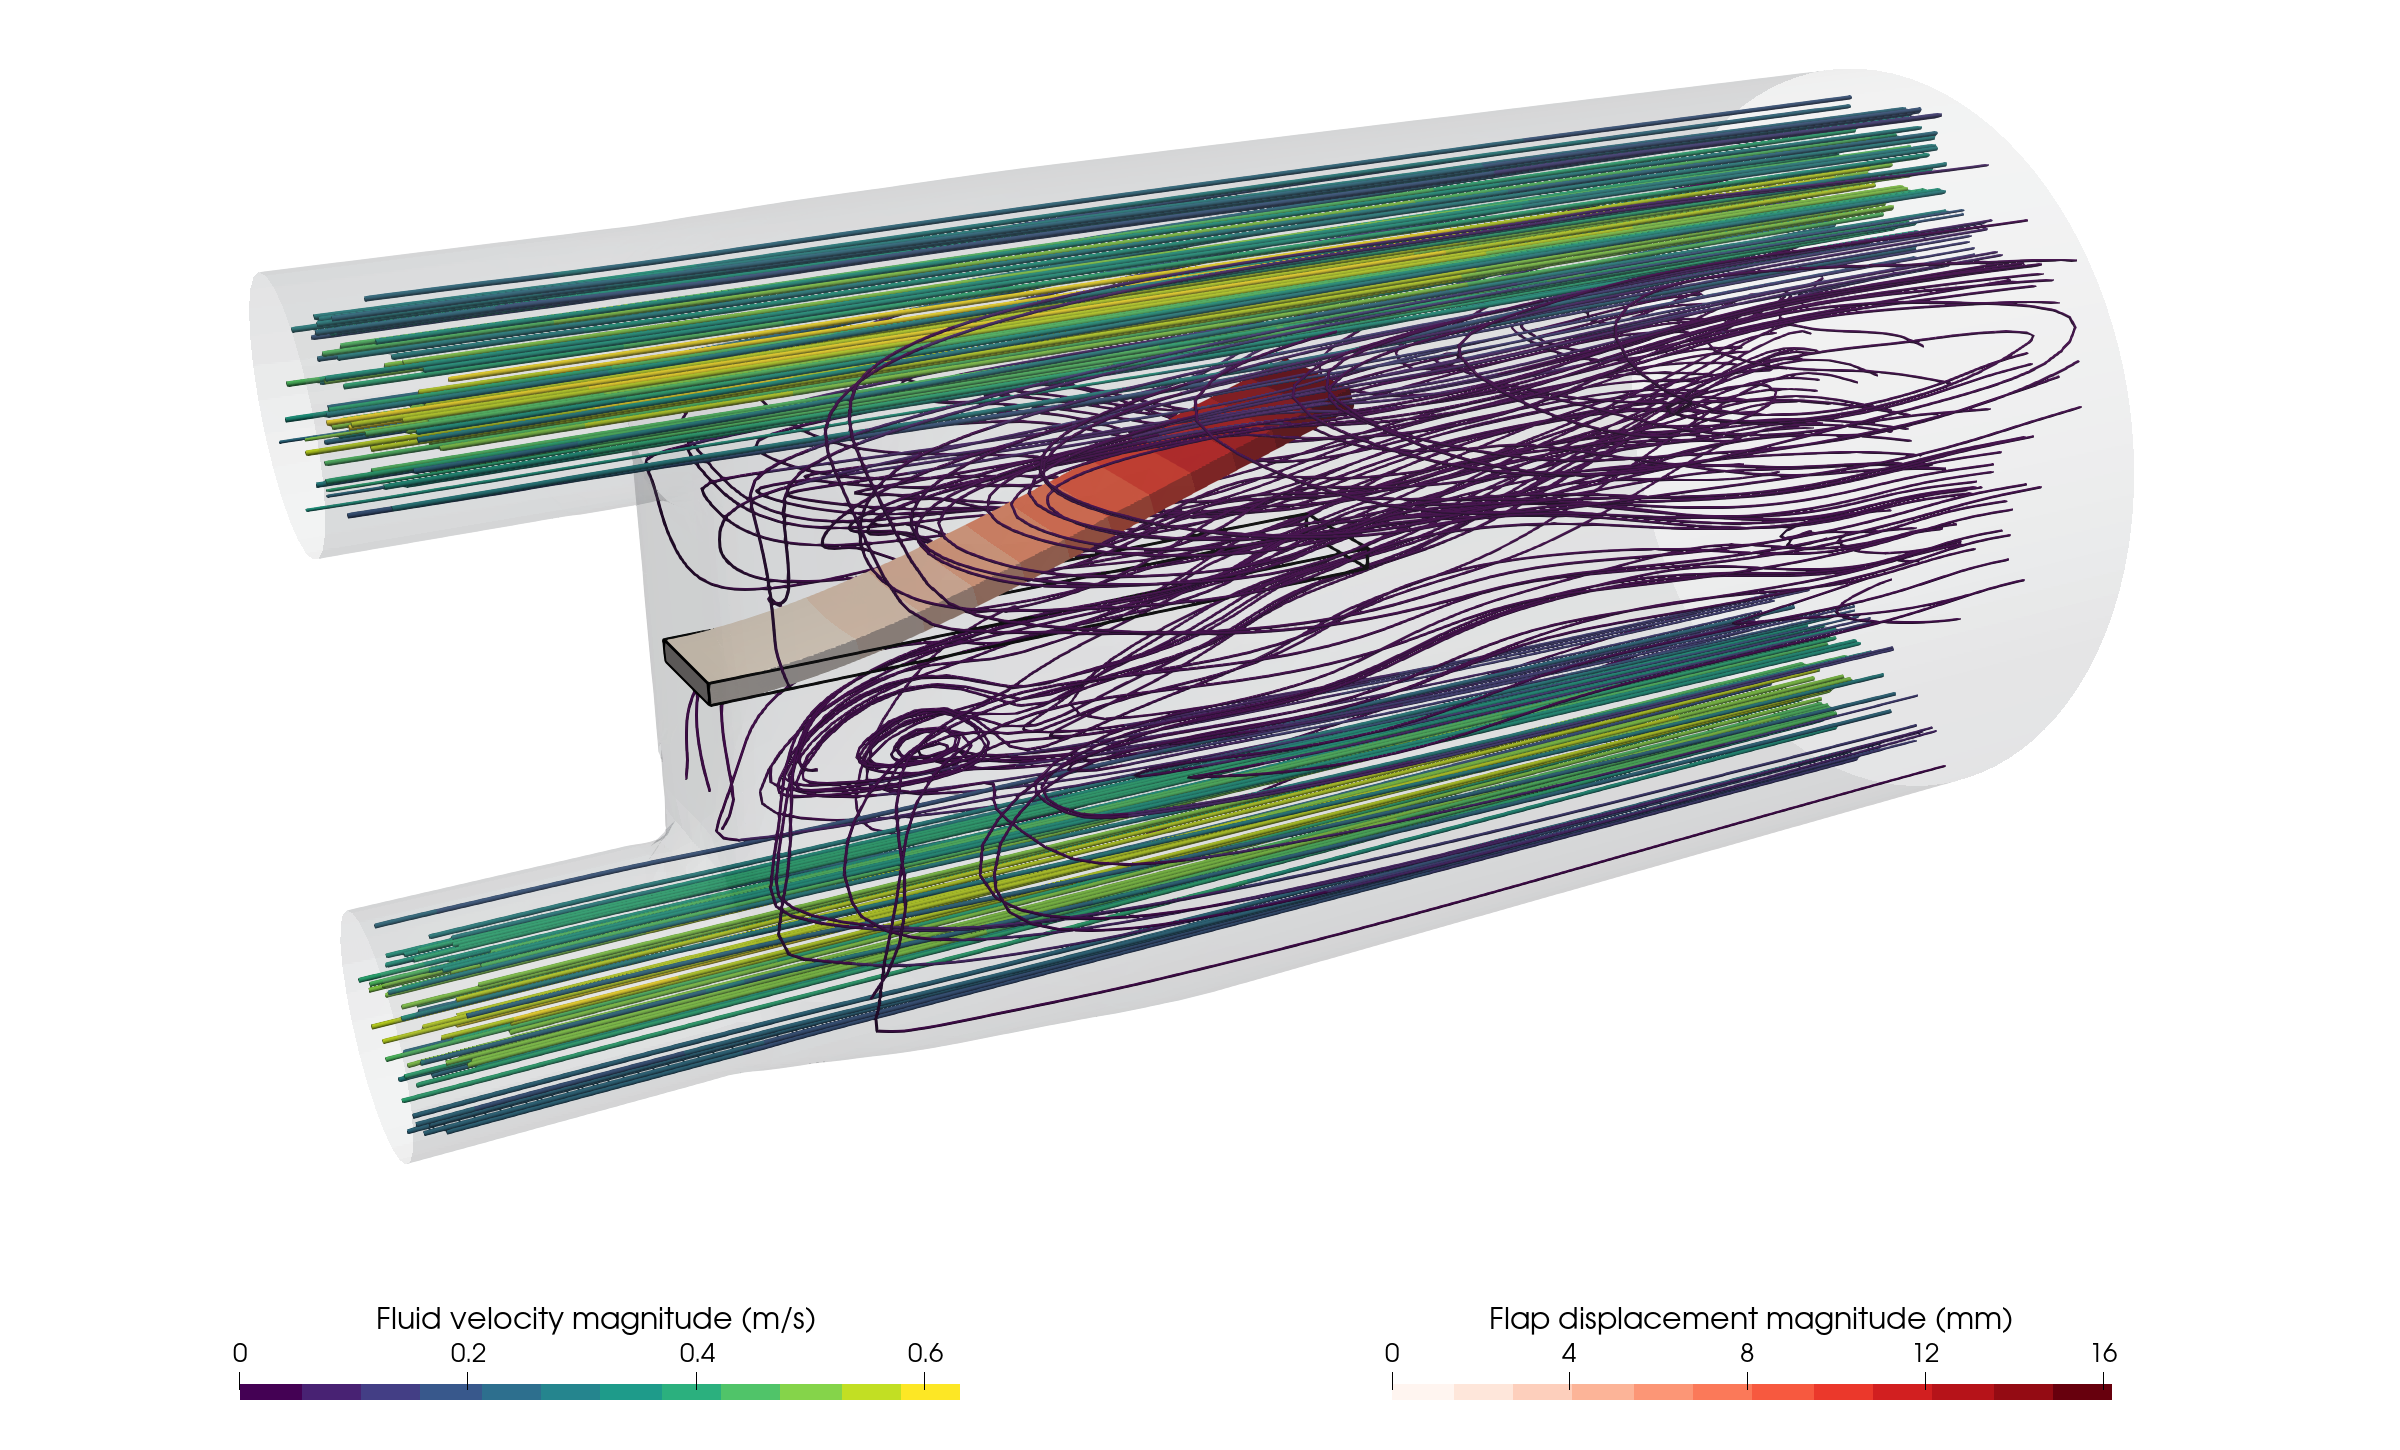
\includegraphics[width=\textwidth]{figures/hessenthaler-3d}
	\caption{Hessenthaler Phase I at steady state ($t = 45\,\mathrm{s}$), quasi-monolithic coupling, rF0 mesh: streamlines coloured by the fluid velocity magnitude, seeded on both inlets and around the flap, and the deformed flap coloured by its displacement magnitude, with its undeformed outline (black); translucent vessel walls, with the outlet pipe shown to $z = 130\,\mathrm{mm}$.}
	\label{fig:hessenthaler_3d}
\end{figure}

\paragraph{Set-up.}
A silicone flap of $11\times2\times65\,\mathrm{mm}$ is clamped where two inlet pipes of diameter $21.9\,\mathrm{mm}$ join an outlet pipe of diameter $76.2\,\mathrm{mm}$; the flow domain is the published vessel surface with the outlet extended by $250\,\mathrm{mm}$~\citep{Hessenthaler2017a}.
An aqueous glycerol solution ($\rho_F = 1163.3\,\mathrm{kg/m^3}$, $\mu_F = 12.50\,\mathrm{mPa\,s}$) enters both inlets with parabolic profiles of peak velocity $630$ and $615\,\mathrm{mm/s}$ ($Re = 1283$), ramped in over $0.5\,\mathrm{s}$.
The flap ($\rho_S = 1058.3\,\mathrm{kg/m^3}$) is lighter than the fluid: as in~\citet{Hessenthaler2017b}, the fluid is solved without gravity and the buoyancy is applied to the solid as the net body force $(\rho_S - \rho_F)\,\bb{g}/\rho_S$, ramped with the inflow.
Buoyancy alone would lift the tip by $29.5\,\mathrm{mm}$; the measured steady deflection under flow is $16.41\,\mathrm{mm}$.
The outlet has a fixed pressure with the backflow-stabilised traction of the benchmark definition ($\beta = 0.2$~\citep{Hessenthaler2017b}).
The flap is a compressible neo-Hookean solid ($\nu_S = 0.45$, $\mu_S = 64.2\,\mathrm{kPa}$, calibrated against the buoyant deflection without flow~\citep{CardiffFSIVerification2026}) on $12\times8\times65$ hexahedra (6\,240 cells), the same solid mesh for every fluid mesh.
The fluid meshes are three octree meshes generated from the vessel surface with the flap edges captured as feature edges and a refinement box over the region the flap tip sweeps; the cell size at the flap is $0.71$, $0.50$ and $0.36\,\mathrm{mm}$ (rF0--rF2, $1.2$, $3.1$ and $8.3\times10^{5}$ cells), and all three pass the strict mesh checks.
% rF family: hv-remesh/rfamily README (shifted octree, tipSweep box, 1.5 mm
% interface band, improveMeshQuality); linear ratios 1.37-1.39.
Both couplings use second-order backward time integration with $\Delta t = 0.002\,\mathrm{s}$ to $t = 45\,\mathrm{s}$, the \texttt{LUST} convection scheme (three-quarters central, one quarter linear upwind), least-squares gradients and AMI transfer across the non-conformal interface.
The quasi-monolithic coupling uses the total Lagrangian velocity solid ($\alpha_d = 0.01$) and the solid-model mesh motion with quadratic inverse-distance stiffness; the partitioned coupling uses the total Lagrangian displacement solid, a velocity Laplacian mesh motion with the same stiffness, PIMPLE with up to 20 outer correctors, and IQN-ILS with the strict test ($10^{-4}$ on both residual measures) and the modes of the two previous steps.
The partitioned runs use a different solids4foam build from the quasi-monolithic runs, which include the interface correction of Section~\ref{sec:fluid_mesh_motion}.
\todo{Add the Newton and Krylov tolerances of the QM runs (rF case files) as a row of Table~\ref{tab:solver_settings}.}

The two inlet jets stay along the wall of the outlet pipe and pass above and below the flap, which buoyancy lifts into the slow region between them, where the fluid moves at a few centimetres per second (Figures~\ref{fig:hessenthaler_3d} and~\ref{fig:hessenthaler_midplane}); its tip almost reaches the shear layer of the upper jet, and a recirculation forms below its root.
% Field images: figures/scripts/paraview/hessenthaler_{3d,midplane}.py, QM rF0 t = 45 s
% reconstructed (claude-runs/hv-figures/case); rF1 mesh from hv-remesh/rfamily.

\paragraph{Measured.}
The tip deflection $u_y$ is averaged over $t = 40$--$45\,\mathrm{s}$, in which the flow is statistically steady (Figure~\ref{fig:hessenthaler_results}a); the deformed centreline is averaged over the same window and compared with the MRI centreline, and the velocity is averaged over the window and over each MRI voxel ($1.302\times1.302\times6\,\mathrm{mm}$) and compared with the phase-contrast MRI velocities on the planes $z = 10$ and $30\,\mathrm{mm}$, with the difference vector normalised by the inlet peak velocity $630\,\mathrm{mm/s}$~\citep{Hessenthaler2017a}.
\todo{Fix the closing window once all six runs reach $t = 45\,\mathrm{s}$; the partitioned rF2 coupling iterations rise from about four per step to a mean of 18 (up to 60) from $t \approx 38\,\mathrm{s}$, so its closing window must be checked before use.}

\begin{table}[htbp]
	\centering
	\footnotesize
	\setlength{\tabcolsep}{3pt}
	\caption{Hessenthaler Phase I: tip deflection $u_y$ (mean, with the minimum and maximum, over $t = 40$--$45\,\mathrm{s}$; measured $16.41\,\mathrm{mm}$), RMS deviation of the mean centreline from the MRI centreline (MRI voxel $0.98\,\mathrm{mm}$), mean voxel velocity difference from MRI relative to $630\,\mathrm{mm/s}$, and Newton (quasi-monolithic) or coupling (IQN-ILS) iterations per step. Runs not yet at $t = 45\,\mathrm{s}$ show the window $t = 5$--$10\,\mathrm{s}$ (marked${}^{\dagger}$) or a dash.}
	\label{tab:hessenthaler_m}
	\begin{tabular}{llrrrrr}
		\toprule
		Mesh & Coupling & Cells & $u_y$ (mm) & Centreline (mm) & Velocity & Iter. \\
		\midrule
		rF0 & QM      & 122\,435 & $15.97$ ($15.86$--$16.05$) & $0.27$ & $5.2\%$ & 2.0 \\
		    & IQN-ILS &          & $16.31$ ($16.28$--$16.32$) & $0.19$ & $5.1\%$ & 4.2 \\
		rF1 & QM      & 312\,180 & $16.45^{\dagger}$          & --     & --      & 2.0 \\
		    & IQN-ILS &          & $16.66$ ($16.64$--$16.68$) & $0.28$ & $4.9\%$ & 4.6 \\
		rF2 & QM      & 832\,552 & --                         & --     & --      & 2.0 \\
		    & IQN-ILS &          & --                         & --     & --      & 18.2 \\
		\bottomrule
	\end{tabular}
\end{table}

\begin{figure}[htbp]
	\centering
	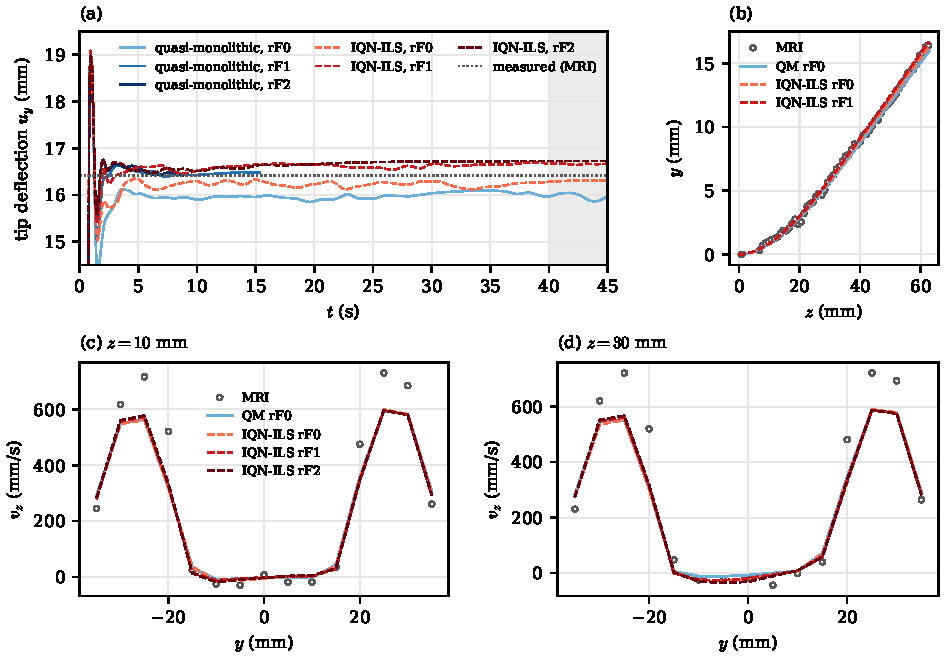
\includegraphics[width=\textwidth]{figures/hessenthaler-results}
	\caption{Hessenthaler Phase I, quasi-monolithic (blue, solid) and IQN-ILS (red, dashed) on the meshes rF0--rF2 (light to dark): (a) tip deflection, with the averaging window shaded and the measured steady value dotted; (b) mean deformed centreline over $t = 40$--$45\,\mathrm{s}$ against MRI; (c, d) mean axial velocity on the line $x = 0$ of the MRI planes $z = 10$ and $30\,\mathrm{mm}$, averaged over each MRI voxel, against phase-contrast MRI.}
	\label{fig:hessenthaler_results}
\end{figure}

\begin{figure}[htbp]
	\centering
	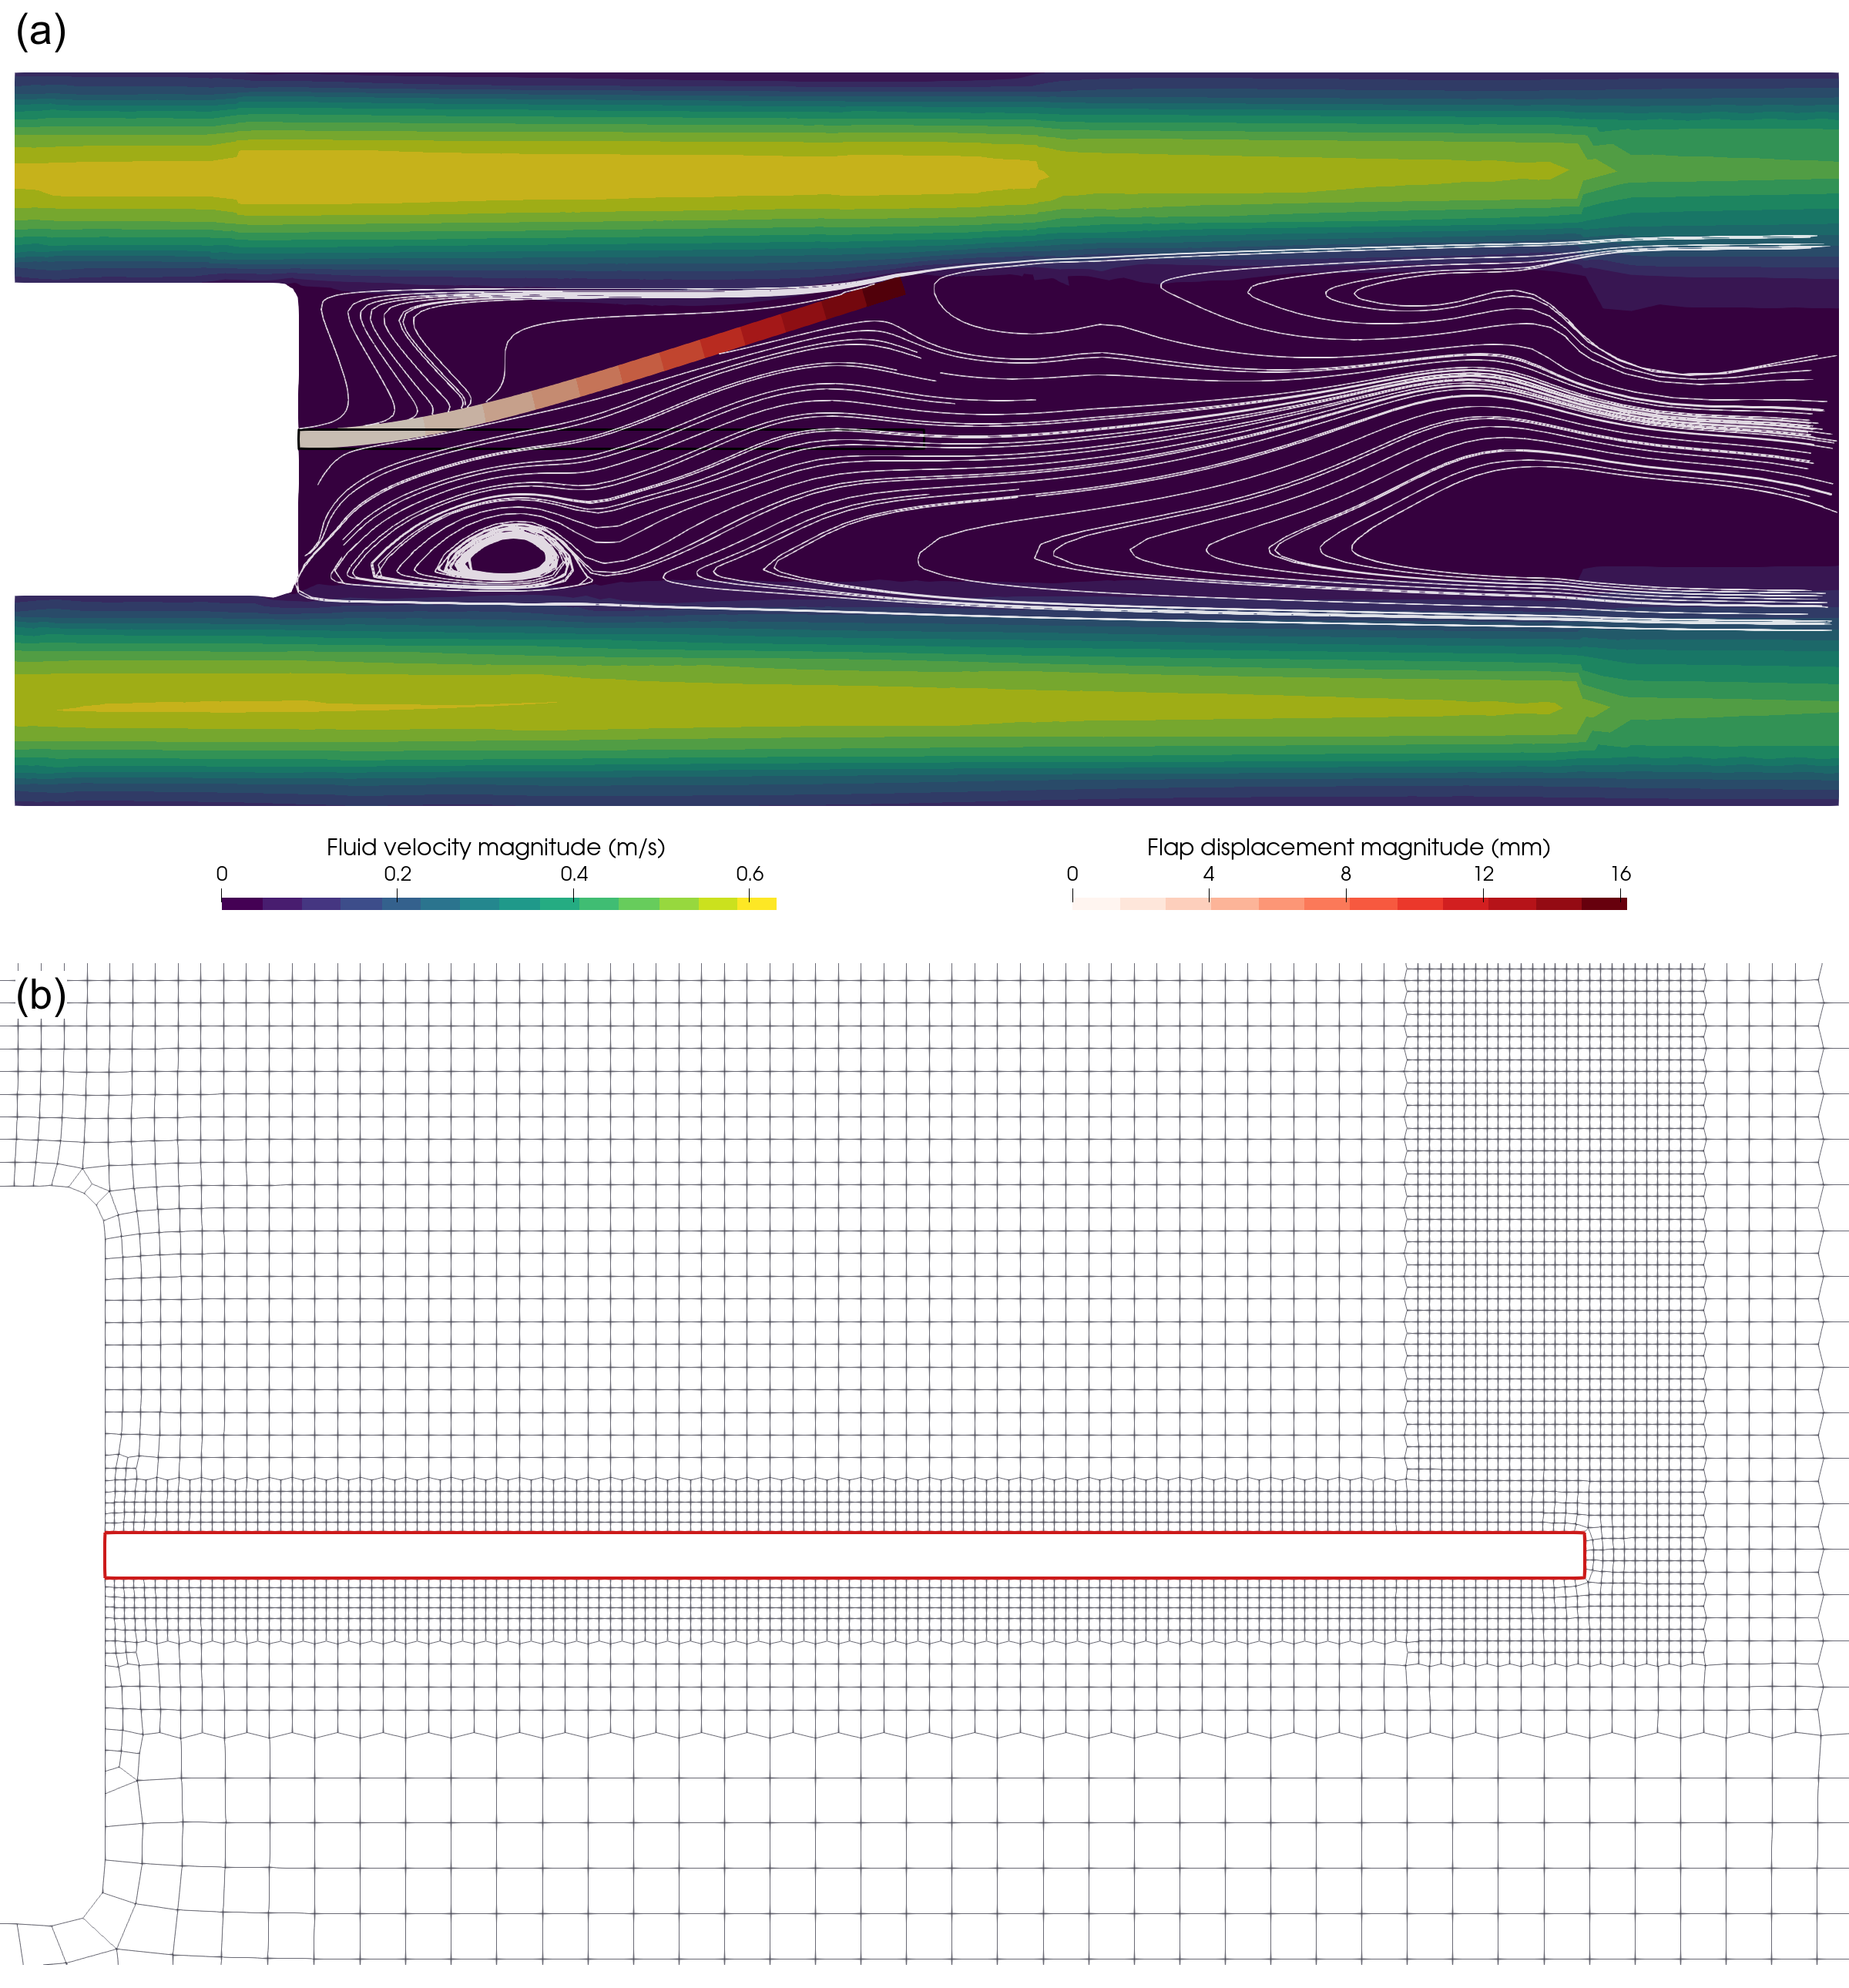
\includegraphics[width=\textwidth]{figures/hessenthaler-midplane}
	\caption{Hessenthaler Phase I: (a) velocity magnitude on the plane $x = 0.3\,\mathrm{mm}$ at $t = 45\,\mathrm{s}$ (quasi-monolithic coupling, rF0 mesh), with in-plane streamlines (white) in the slow central region and the deformed flap coloured by its displacement magnitude, with its undeformed outline (black), for $-30 \le z \le 160\,\mathrm{mm}$; (b) the rF1 fluid mesh on the same plane near the flap, with the undeformed flap (red), the refined band around the flap and the refinement box over the region the tip sweeps.}
	\label{fig:hessenthaler_midplane}
\end{figure}

\paragraph{Comparison of the couplings.}
The quasi-monolithic coupling needs two Newton iterations per step on every mesh and throughout the run (three in 2, 1 and 22 steps of the first $5\,\mathrm{s}$ on rF0--rF2), including the first second, in which the flap swings up to a tip deflection of $19\,\mathrm{mm}$ and back (Figure~\ref{fig:hessenthaler_results}a).
IQN-ILS needs about four coupling iterations per step on rF0 and rF1; on rF2 it needs four until $t \approx 35\,\mathrm{s}$, after which the count rises to a mean of 18 per step over $t = 40$--$42.4\,\mathrm{s}$ with steps at the limit of 60.
% P_rF2 fsiResiduals: mean per 5 s window 4.1, 4.0, 4.0, 4.0, 4.0, 4.3, 4.5, 8.4, 18.2.
On rF0 the closing-window tip deflection is $15.97\,\mathrm{mm}$ with the quasi-monolithic coupling and $16.31\,\mathrm{mm}$ with IQN-ILS, $2.1\%$ apart; over $t = 5$--$10\,\mathrm{s}$, the window both couplings have reached on rF0 and rF1, the difference falls from $1.6\%$ on rF0 to $0.6\%$ on rF1 ($15.95$ against $16.21$, and $16.45$ against $16.55\,\mathrm{mm}$).
The couplings thus approach each other under refinement, as on the two-dimensional cases, where they differ by the discretisation differences of Section~\ref{sec:consistency_partitioned}, here in particular the velocity against the displacement solid and the mesh moved once per step against once per coupling iteration.
The partitioned tip deflection changes by $0.40\,\mathrm{mm}$ from rF0 to rF1 and by $0.07\,\mathrm{mm}$ from rF1 to rF2 (over $t = 20$--$25\,\mathrm{s}$, $16.21$, $16.61$ and $16.68\,\mathrm{mm}$): on rF0 the fluid-mesh error, about $3\%$, exceeds the difference between the couplings, whereas on rF1 the two are of similar size ($0.4$ and $0.6\%$).
\todo{Complete with the QM rF1 and rF2 closing-window values and, if the sequence is monotone, the observed order and the extrapolated deflection for both couplings.}

\paragraph{Comparison with the measurements.}
On every mesh and with both couplings the tip deflection lies within $0.5\,\mathrm{mm}$ of the measured $16.41\,\mathrm{mm}$, and the mean centreline deviates from the MRI centreline by $0.2$--$0.3\,\mathrm{mm}$ RMS, less than a third of the MRI voxel size (Figure~\ref{fig:hessenthaler_results}b).
The voxel-averaged velocities differ from the MRI velocities by $5\%$ of the inlet peak on average, with both couplings and on both meshes compared; the two couplings differ from each other by much less (Figure~\ref{fig:hessenthaler_results}c, d).
The largest differences are at the jet cores, where both couplings predict $595\,\mathrm{mm/s}$ against the measured $731\,\mathrm{mm/s}$ on the plane $z = 10\,\mathrm{mm}$; since the couplings agree there to $1\%$, this difference belongs to the shared model (inflow profiles, geometry) or to the measurement, not to the coupling.
% Jet-core voxel (z = 10, y = 25): MRI 730.5, QM rF0 594.8, IQN rF0 599.1, rF1 596.9 mm/s.
\todo{The measured velocities exceed the prescribed inflow peak of $630\,\mathrm{mm/s}$ at the jet cores; check against the inflow definition of~\citet{Hessenthaler2017a,Hessenthaler2017b} before discussing.}

\paragraph{Cost.}
The quasi-monolithic runs took $2470$, $8070$ and $14\,600\,\mathrm{s}$ of elapsed time per simulated second on 64, 96 and 256 MeluXina processes on rF0, rF1 and rF2 ($44$, $215$ and $1040$ core-hours per simulated second); these runs did not follow the timing protocol of Section~\ref{sec:protocol}.
% QM elapsed from ExecutionTime over t >= 5 s: rF0 98790 s for t 5-45, rF1
% 83853 s for 5-15.39, rF2 54858 s for 5-8.75.
The partitioned runs ran on a different cluster, and timings from different machines are not compared.
\todo{Protocol timings of both couplings on MeluXina (restart from a saved state, exclusive node, one window of steps, median of three) on rF0 and rF1, to give the cost ratio at equal mesh.}
